\documentclass[titlepage,a4paper]{jsarticle}
\usepackage{../../sty/import}% 各種パッケージインポート
\usepackage{../../sty/title}% タイトルページの変更
\usepackage{longtable}
\renewcommand{\thesection}{課題\arabic{section}}
\renewcommand{\thesubsection}{問題\arabic{subsection}}
\renewcommand{\thesubsubsection}{(\arabic{subsubsection})}
%% タイトルページの変数
% レポートタイトル
\title{統計工学課題}
% 提出日
\expdate{\today}
% 科目名
\subject{統計工学}
% 分野
\class{情報経営システム工学分野}
% 学年
\grade{B3}
% 学籍番号
\mynumber{24336488}
% 記述者
\author{本間 三暉}

\begin{document}
% titleページ作成
\maketitle

\section{ }%% 課題1
\subsection{記述統計}
\subsection*{以下の表\ref{tab:kabuto}はある地域に生息するオスのカブトムシの体長と角長の測定結果である。}
\begin{longtable}{|c|c|c|}
  \caption{カブトムシ調査結果}
  \label{tab:kabuto}        \\
  \hline
  個体 No & 体長 (mm) & 角長 (mm) \\ \hline
  \endhead
  1     & 33.2    & 14.5    \\ \hline
  2     & 38.1    & 15.1    \\ \hline
  3     & 42.6    & 21.5    \\ \hline
  4     & 45.3    & 22.4    \\ \hline
  5     & 49.2    & 16.3    \\ \hline
  6     & 50.6    & 22.5    \\ \hline
  7     & 51.7    & 21.8    \\ \hline
  8     & 54.8    & 24.9    \\ \hline
  9     & 57.1    & 25.4    \\ \hline
  10    & 60.2    & 15.6    \\ \hline
  11    & 61.8    & 25.1    \\ \hline
  12    & 64.3    & 45.2    \\ \hline
  13    & 68.5    & 45.3    \\ \hline
  14    & 68.9    & 32.6    \\ \hline
  15    & 69.1    & 32.4    \\ \hline
  16    & 69.3    & 35.4    \\ \hline
  17    & 75.5    & 41.6    \\ \hline
  18    & 75.7    & 42.6    \\ \hline
  19    & 77.6    & 41.4    \\ \hline
  20    & 78.1    & 45.6    \\ \hline
  21    & 78.5    & 46.2    \\ \hline
  22    & 79.2    & 45.8    \\ \hline
  23    & 79.3    & 45.4    \\ \hline
  24    & 84.8    & 47.9    \\ \hline
  25    & 87.6    & 48.6    \\ \hline
  26    & 88.1    & 50.7    \\ \hline
  27    & 89.1    & 49.3    \\ \hline
  28    & 89.6    & 52.3    \\ \hline
  29    & 97.5    & 51.4    \\ \hline
  30    & 98.8    & 51.2    \\ \hline
\end{longtable}
\subsubsection{体長、角長をそれぞれ解析せよ(度数分布表、ヒストグラム、平均、分散、標準偏差を求め、結果について考察する)。}\label{toi1_1_1}
体長と角長の度数分布表をそれぞれ表\ref{tab:frequency1}と表\ref{tab:frequency2}に示す.
\begin{longtable}{|c|c|c|c|c|c|c|}
  \caption{体長の度数分布表} \label{tab:frequency1}                                                                \\
  \hline
  \textbf{以上} & \textbf{未満} & \textbf{階級値} & \textbf{度数} & \textbf{累積度数} & \textbf{相対度数} & \textbf{累積相対度数} \\ \hline
  \endfirsthead
  \hline
  \textbf{以上} & \textbf{未満} & \textbf{階級値} & \textbf{度数} & \textbf{累積度数} & \textbf{相対度数} & \textbf{累積相対度数} \\ \hline
  \endhead
  30          & 40          & 35           & 2           & 2             & 0.067         & 0.067           \\ \hline
  40          & 50          & 45           & 3           & 5             & 0.100         & 0.167           \\ \hline
  50          & 60          & 55           & 4           & 9             & 0.133         & 0.300           \\ \hline
  60          & 70          & 65           & 7           & 16            & 0.233         & 0.533           \\ \hline
  70          & 80          & 75           & 7           & 23            & 0.233         & 0.767           \\ \hline
  80          & 90          & 85           & 5           & 28            & 0.167         & 0.933           \\ \hline
  90          & 100         & 95           & 2           & 30            & 0.067         & 1.000           \\ \hline
\end{longtable}

\begin{longtable}{|c|c|c|c|c|c|c|}
  \caption{角長の度数分布表} \label{tab:frequency2}                                                                \\
  \hline
  \textbf{以上} & \textbf{未満} & \textbf{階級値} & \textbf{度数} & \textbf{累積度数} & \textbf{相対度数} & \textbf{累積相対度数} \\ \hline
  \endfirsthead
  \hline
  \textbf{以上} & \textbf{未満} & \textbf{階級値} & \textbf{度数} & \textbf{累積度数} & \textbf{相対度数} & \textbf{累積相対度数} \\ \hline
  \endhead
  10          & 20          & 15           & 4           & 4             & 0.133         & 0.133           \\ \hline
  20          & 30          & 25           & 7           & 11            & 0.233         & 0.367           \\ \hline
  30          & 40          & 35           & 3           & 14            & 0.100         & 0.467           \\ \hline
  40          & 50          & 45           & 12          & 26            & 0.400         & 0.867           \\ \hline
  50          & 60          & 55           & 4           & 30            & 0.133         & 1.000           \\ \hline
\end{longtable}
体長と角長のヒストグラムをそれぞれ図\ref{fig:image1},図\ref{fig:image2}に示す.
\begin{figure}[h]
  \centering
  % 左側の画像
  \begin{subfigure}{0.45\textwidth}
    \centering
    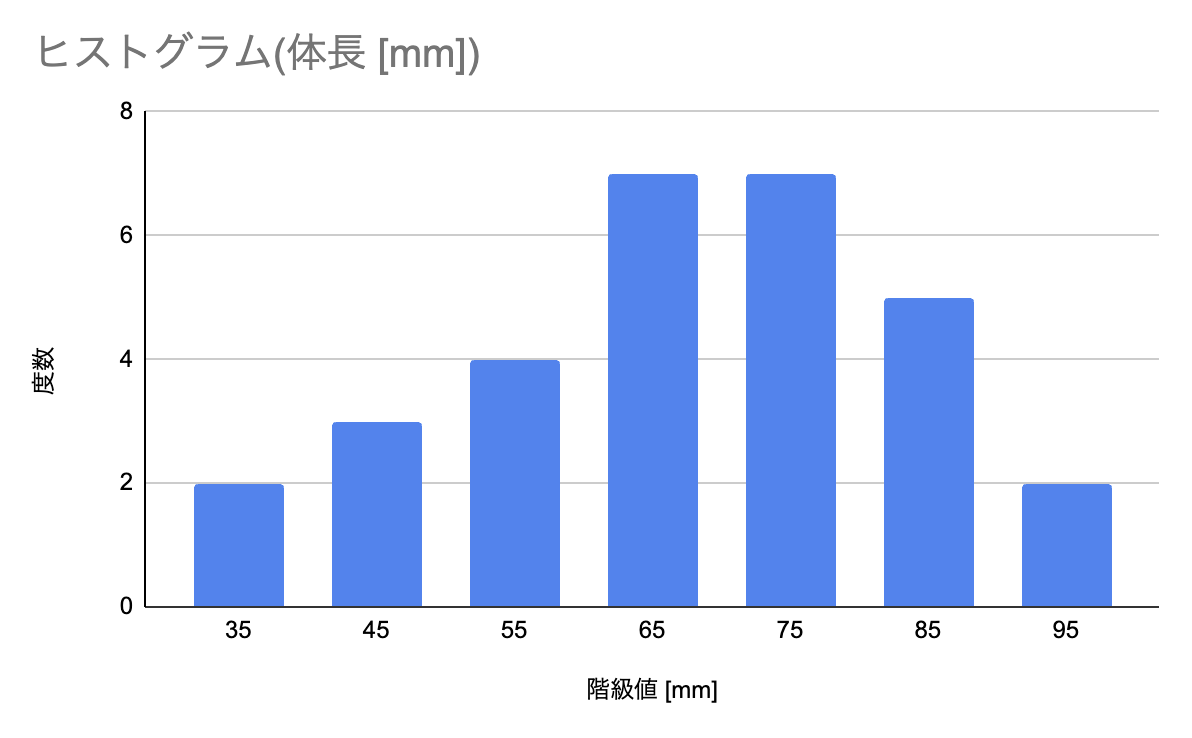
\includegraphics[width=\textwidth]{img/TT_hist.png}
    \caption{体長のヒストグラム}
    \label{fig:image1}
  \end{subfigure}
  % 右側の画像
  \begin{subfigure}{0.45\textwidth}
    \centering
    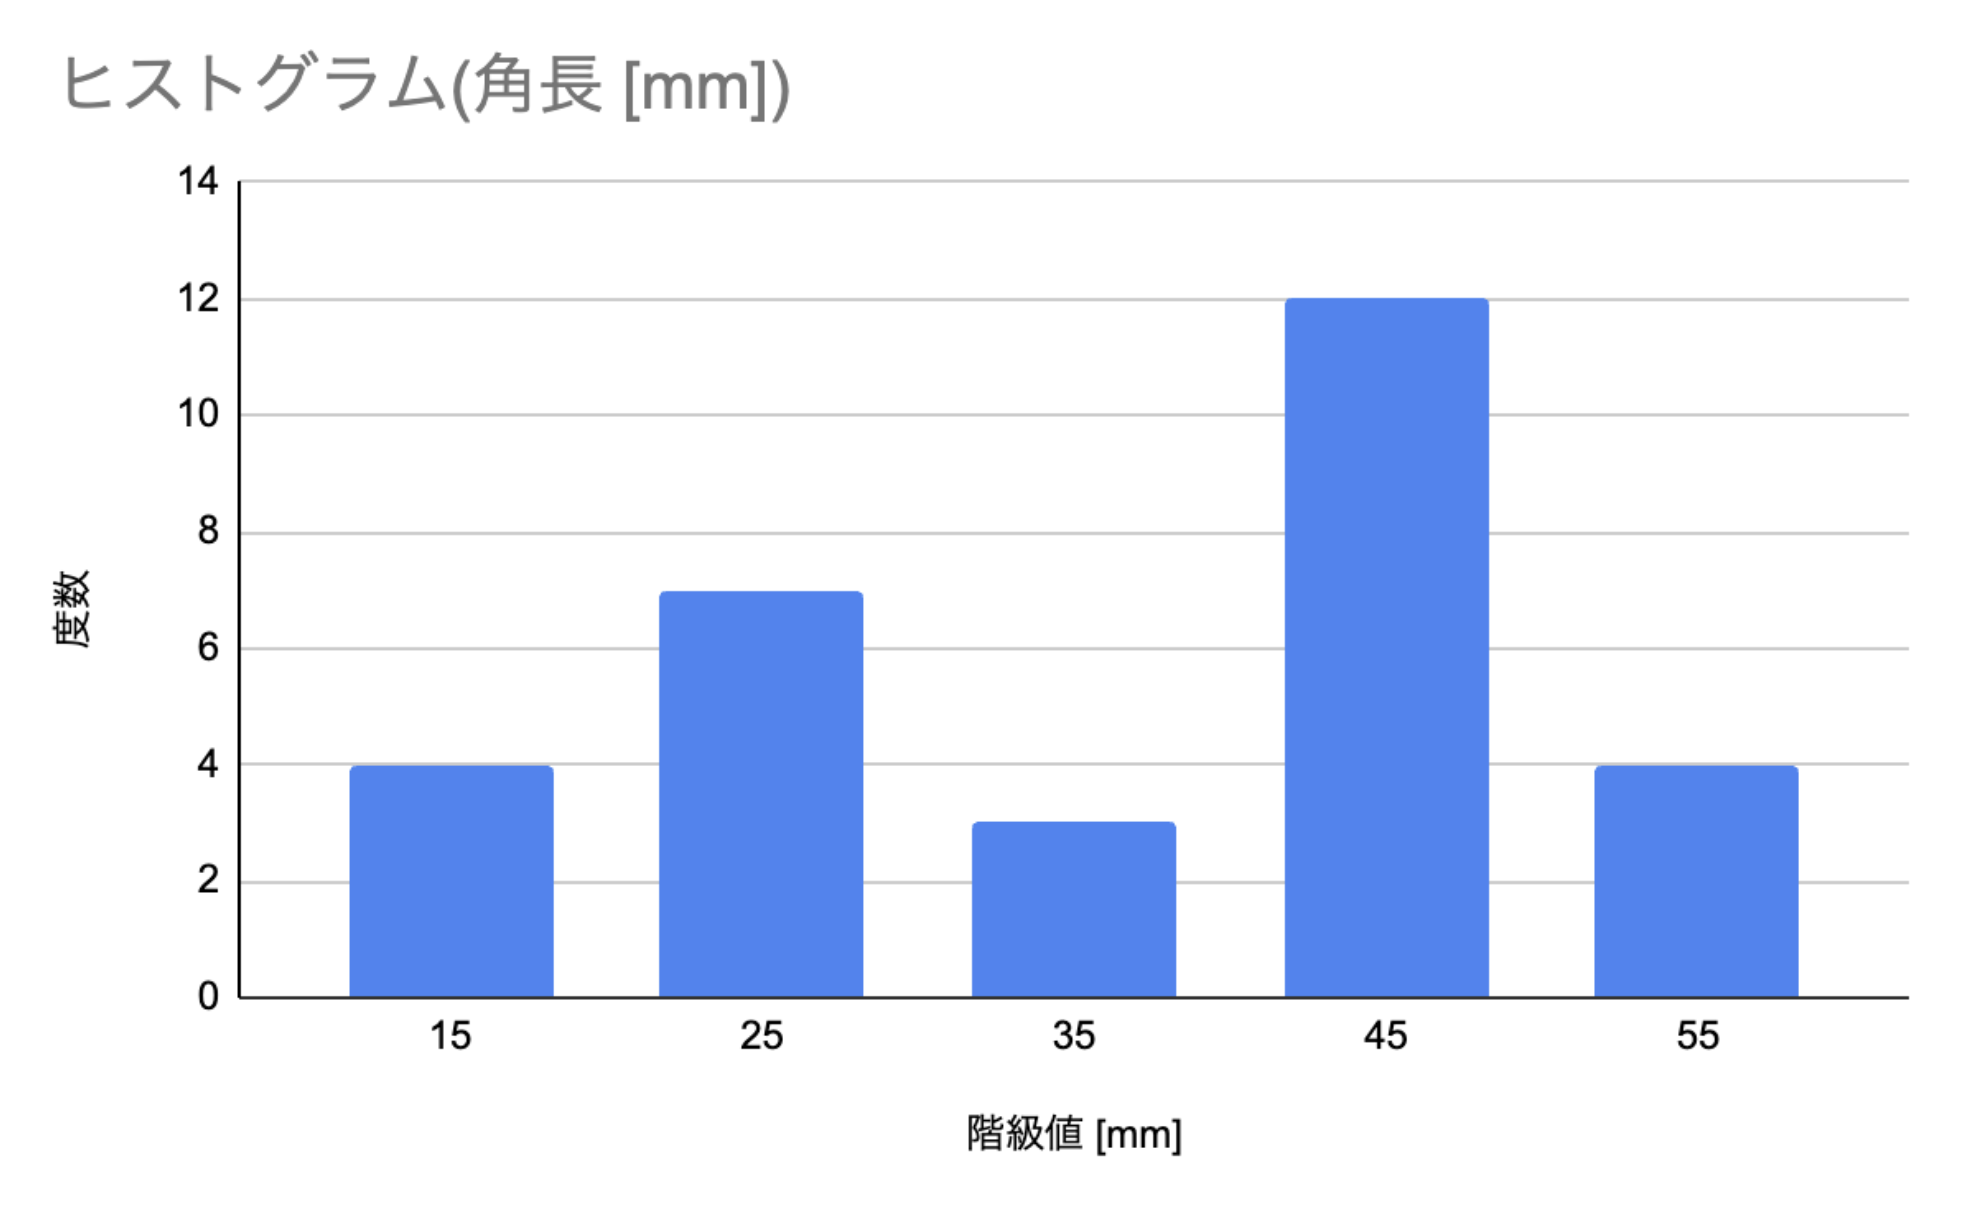
\includegraphics[width=\textwidth]{img/KT_hist.png}
    \caption{角長のヒストグラム}
    \label{fig:image2}
  \end{subfigure}
  \caption{カブトムシのヒストグラム}
  \label{fig:side_by_side_images}
\end{figure}

表\ref{tab:statistics}に体長と角長の平均,分散,標準偏差を示す.
データは,ある地域に生息する押すのカブトムシの測定結果であり,標本調査なので,分散と標準偏差は不偏分散と普遍標準偏差を求めた.
\begin{longtable}{|c|c|c|}
  \caption{体長と角長の統計量} \label{tab:statistics}      \\ \hline
  \textbf{} & \textbf{体長 (mm)} & \textbf{角長 (mm)} \\ \hline
  \endfirsthead
  \hline
  \textbf{} & \textbf{体長 (mm)} & \textbf{角長 (mm)} \\ \hline
  \endhead
  平均        & 68.80            & 35.87            \\ \hline
  分散        & 301.74           & 164.81           \\ \hline
  標準偏差      & 17.37            & 12.84            \\ \hline
\end{longtable}

ヒストグラムから,体長は65[mm]から75[mm]を中心に大きな山となっていて,角長は25[mm]と45[mm]の2つの山に分布していることがわかる.
また,データから角長より体長の値のほうが広範囲に分布していることがわかる.
体長と角長のデータより,体長の小さい個体は角長が小さく,体長の大きい個体は角長が大きいことが予想できる.
また,体長が1つの山に固まっているのに対し,角長が2つの山になっていることと,特定地域のオスの個体の標本であることから,
成長段階の違う個体を測定していることが考えられるが,これらのデータだけでは断言することはできない.
\subsubsection{体長と角長の関係について調べよ(散布図、共分散、相関係数を求め、結果について考察する)}
図\ref{fig:sanp}に体長と角長の散布図を示す.
\begin{figure}[H]
  \centering
  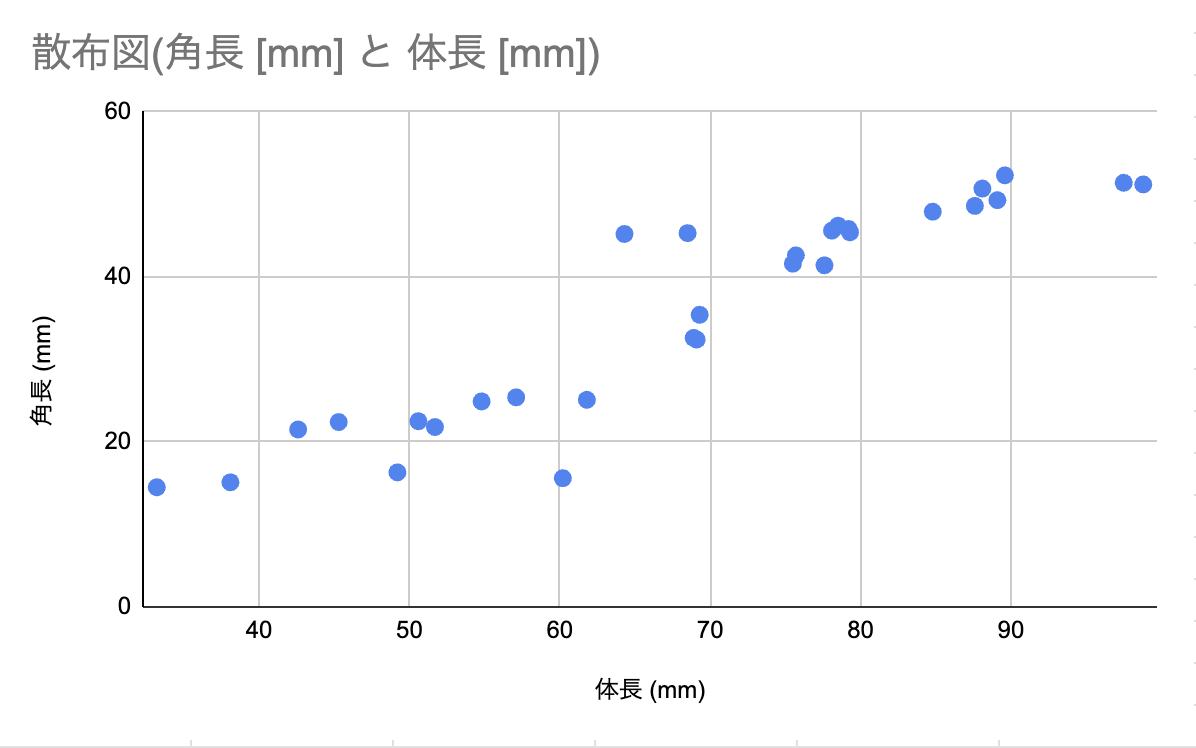
\includegraphics[width=0.8\textwidth]{img/sanp.png}
  \caption{散布図}
  \label{fig:sanp}
\end{figure}

表\ref{tab:covariance_correlation}に共分散と相関係数を示す.
\begin{longtable}{|c|c|}
  \caption{共分散と相関係数} \label{tab:covariance_correlation} \\ \hline
  \textbf{項目} & \textbf{値}                              \\ \hline
  \endfirsthead
  \hline
  \textbf{項目} & \textbf{値}                              \\ \hline
  \endhead
  共分散         & 206.80                                  \\ \hline
  相関係数        & 0.93                                    \\ \hline
\end{longtable}

まず,相関係数が0.93なので,体長と角長には強い正の相関があることがわかる.
また,図\ref{fig:sanp}より,グラフ左下と右上の2グループに分かれているように見えることから,
\ref{toi1_1_1}で考察した内容と被る部分もあるが,体長の小さい個体は角長が小さく,
体長の大きい個体は角長が大きいことが分かり,成長段階の違う個体を測定しているためこのような結果が現れるのではないかと考えられる.

\subsubsection*{メモ}

\textbf{共分散の定義}\\
共分散の定義は式\eqref{siki1}のように定義される.
これは2変量が $xy$ 平面でどのように散らばっているかを表す.
\begin{equation}
  S_{xy} = \frac{1}{n} \sum_{i=1}^n (x_i - \bar{x})(y_i - \bar{y})\label{siki1}
\end{equation}


\vspace{1em} % 少し余白を追加

\textbf{相関係数の定義}\\
対応のある2変量 $x, y$ について,式\eqref{siki2}を $x$ と $y$ の相関係数という.
\begin{equation}
  r = \frac{S_{xy}}{s_x \cdot s_y}\label{siki2}
\end{equation}


\subsection{確率}
\subsection*{コインを 3 回投げる試行で、\\
  \hspace{1em} 事象 A:1回目に表がでる\\
  \hspace{1em} 事象 B:3回とも同じ側が出る\\
  とするとき、次の確率を求めなさい。
}
事象AとBについてそれぞれの確率$P(A)$,$P(B)$の値を式\eqref{pa}と式\eqref{pb}に示す.
\begin{align}
  P(A) & = \frac{1}{2}  \label{pa}                             \\
  P(B) & = \frac{2}{2^3} = \frac{2}{8} = \frac{1}{4}\label{pb}
\end{align}
\subsubsection{$P(A \cup B)$}
$P(A \cup B)$は事象AかBのどちらか一方は必ず起こる確率である.
事象Aは一回目に表が出ること,事象Bは三回とも同じ側が出ることなので,式\eqref{a_b}に示すように,これらの確率を足し合わせ,重複する部分を引いた値が解となる.
\begin{equation}
  P(A) + P(B) - P(A \cap B) = \frac{1}{2} + \frac{1}{4} - \frac{1}{8} = \frac{5}{8}\label{a_b}
\end{equation}

\subsubsection{$P(\overline{A})$}
\begin{equation}
  P(\overline{A})=1-P(A)=1-\frac{1}{2}=\frac{1}{2}
\end{equation}
\subsubsection{$P(\overline{B})$}
\begin{equation}
  P(\overline{B})=1-P(B)=1-\frac{1}{4}=\frac{3}{4}
\end{equation}

\subsection{確率}
\subsection*{袋に当たりくじ1枚とハズレくじ5枚が入っており、2人で交互に 1枚ずつくじを取り出すとする。
  引いたくじは戻さないとき、先に引き始めた者と、後から引き始めた者とではどちらが得か?}
まず,n回目にくじを引いたときあたりを引く確率を$P_n$とすると,今回あり得る事象の確率は式\eqref{p1}から式\eqref{p6}の式の内どれかで表せる.
\begin{align}
  P_1 & = \frac{1}{6} \label{p1}                                                                                                              \\
  P_2 & = \frac{5}{6} \times \frac{1}{5} = \frac{1}{6} \label{p2}                                                                             \\
  P_3 & = \frac{5}{6} \times \frac{4}{5} \times \frac{1}{4} = \frac{1}{6} \label{p3}                                                          \\
  P_4 & = \frac{5}{6} \times \frac{4}{5} \times \frac{3}{4} \times \frac{1}{3} = \frac{1}{6} \label{p4}                                       \\
  P_5 & = \frac{5}{6} \times \frac{4}{5} \times \frac{3}{4} \times \frac{2}{3} \times \frac{1}{2} = \frac{1}{6} \label{p5}                    \\
  P_6 & = \frac{5}{6} \times \frac{4}{5} \times \frac{3}{4} \times \frac{2}{3} \times \frac{1}{2} \times \frac{1}{1} = \frac{1}{6} \label{p6}
\end{align}

つまり,それぞれのくじが引かれるかどうかが同様に確からしい場合,いつ引いても確率は変わらない.
そのため,引く回数が同じ場合どちらも同じ確率であたりを引く可能性があるため,引く順番による差は無いと言える.

余談だが,これはくじを引く前に考えているためすべて同じ確率となるが,くじを引いた結果があらかじめ分かってしまうと確率が変わってしまう.

\subsubsection*{メモ}
\textbf{排反事象}\\
事象A,Bが背反 → $A \cup B = \phi $

$P(A \cap B)=P(A)+P(B)-P(A \cup B)$のうち,$P(A\cup B)=0$となる.

\subsection{確率と条件付き確率}
\subsection*{サイコロを2回振るとき、次の確率を求めなさい。}
サイコロを2回振る場合の目の組み合わせは$6 \times 6=36$通りである.
\subsubsection{目の和が偶数である確率}
和が偶数となる目の組み合わせは,偶数+偶数か,奇数+奇数の場合である.
これを事象Aとすると,事象Aが起こり得るサイコロの組み合わせは式\eqref{4_n_a},その時の確率は式\eqref{4_p_a}と表せる.
\begin{align}
  n(A) = (3 \times 3)+(3 \times 3)=18\text{通り}\label{4_n_a} \\
  P(A) = \frac{n(A)}{6\times6} = \frac{18}{36} = \frac{1}{2}\label{4_p_a}
\end{align}
\subsubsection{目の和が3の倍数である確率}
サイコロの出る目を3で割ったときのあまりとしてあり得る組み合わせは0,1,2の3通りとなる.
その時,和が3の倍数となるあまりの組み合わせは(0,0),(1,2),(2,1)の3通りである.

また,2つのサイコロのあまりの組み合わせは$3 \times 3=9$通りであるので,3の倍数となるあまりの組み合わせとなる確率は$\frac{3}{9}=\frac{1}{3}$となる.

したがって,2つのサイコロの目の和が3の倍数になる事象をBとしたときの確率は,$P(B)=\frac{1}{3}$となる.
\subsubsection{目の和が偶数であるとき、目の和が3の倍数でもある確率}
事象AとBは独立なので,式\eqref{4ba}で表せる.
\begin{align}
  P_A(B)=\frac{P(A \cap B)}{P(A)}=\frac{P(B) \times P(A)}{P(A)} =P(B)=\frac{1}{3}\label{4ba}
\end{align}
\subsubsection{目の和が3の倍数であるとき、目の和が偶数でもある確率}
事象AとBは独立なので,式\eqref{4ab}で表せる.
\begin{align}
  P_B(A)=\frac{P(A \cap B)}{P(B)}=\frac{P(A) \times P(B)}{P(B)} =P(A)=\frac{1}{3}\label{4ab}
\end{align}

\subsection{条件付き確率}
\subsubsection*{あるお店で次のようなゲームが行われている。
  3つの箱があり、うち1つの箱には豪華商品が入っており、ほか2つの箱は空である。
  客はこの中から1つの箱を選び、もし商品が入っていたらもらうことができる。
  ただし、箱を1つ選んだ後、残りの2つのうち空の箱を店員が開け、選ぶ箱を変更するかどうかを尋ねてくる(残り2つの両方が空の場合、無作為に開ける)。
  変更したほうがよいかどうか、答えよ。}
この問題は,モンティ・ホール問題を模した問題であると考えられる.
モンティ・ホール問題は選ぶ箱は変更した方が変える前の2倍当たりやすくなることで知られているが,計算で求めようと思う.

それぞれの箱をA,B,Cとしたとき,プレイヤーはAの箱を選び,司会者がBの箱を開けたと仮定する.
この状況を$E$としたとき,$E$の状況下で箱A,B,Cが当たりであるという事象をそれぞれ事象A,B,Cとすると,
$P(A)=P(B)=P(C)=\frac{1}{3}$であり,求める確率は式\eqref{monty_baiz}で表せる.
\begin{align}
  P_E(A)=\frac{P(A\cap E)}{P(E)}\label{monty_baiz}
\end{align}

$P(A \cap B)=P(A)P_A(E)$について,Aが正解であれば,BとCのどちらも外れとなり,
Bが開けられる確率は$\frac{1}{2}$であるから,$P_A(E)=\frac{1}{2}$となる.
よって,$P(A \cap E) = \frac{1}{3} \times \frac{1}{2} = \frac{1}{6}$となる.

$P(B \cap E) = P_B(E) P(B)$ について,$B$ が正解の場合,$E$ は起こらない($B$ のドアは開かない)ので,$P_B(E) = 0$.
よって,$P(B \cap E) = 0$となる.

$P(C \cap E) = P_C(E) P(C)$ について,$C$ が正解であれば司会者は必ず $B$ を開ける必要があるので,$P_C(E) = 1$ であるから,$P_C(E) = 1$となる.
よって,$P(C \cap E) = \frac{1}{3} \times 1 = \frac{1}{3}$

つまり,
\begin{align}
  P(E) & = P(A \cap E) + P(B \cap E) + P(C \cap E)     \\
       & = \frac{1}{6} + 0 + \frac{1}{3} = \frac{1}{2}
\end{align}
よって,
\begin{align}
  P_E(A) & = \frac{P(A \cap E)}{P(E)} = \frac{\frac{1}{6}}{\frac{1}{2}} = \frac{1}{3}\label{aa} \\
  P_E(B) & = \frac{P(B \cap E)}{P(E)} = 0\label{bb}                                             \\
  P_E(C) & = 1 - P_E(A) - P_E(B) = 1 - \frac{1}{3} - 0 = \frac{2}{3}\label{cc}
\end{align}
となる.
$E$(最初にAを選んでBが開けられた)という条件下では,Aが正解の確率が$\frac{1}{3}$,Bが正解の確率が$0$,
Cが正解の確率が$\frac{2}{3}$なので,箱を変えたほうが当たる確率が2倍になるので変えたほうが良いと言える.

\subsection{ベイズ確率}
\subsection*{X病は3000人に1人の割合で発症する病気であり、この病気に対する第1次血液検査の精度は図\ref{toi6}の通りである。}
\begin{figure}[H]
  \centering
  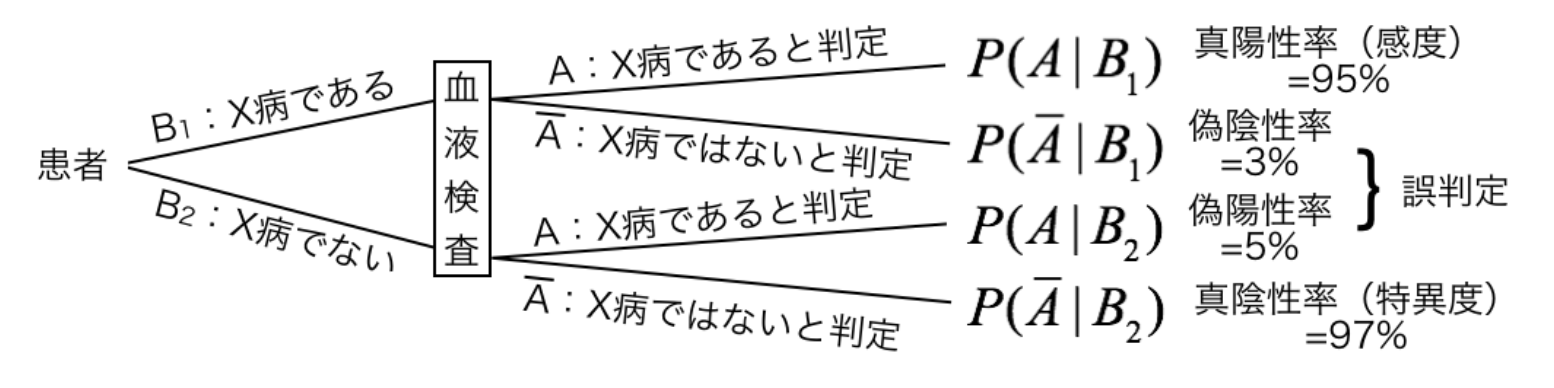
\includegraphics[width=0.8\textwidth]{img/toi6.png}
  \caption{X病に対する第1次血液検査の精度}
  \label{toi6}
\end{figure}
\begin{itemize}
  \item[$A$:] X病であると判定されること(結果が陽性)
  \item[$B_1$:] 実際にX病であること
  \item[$B_2$:] 実際にX病でないこと
\end{itemize}
各事象を上記のように定義する.
\subsubsection{Yさんが1次検査の結果、X病であると判定されたとき、本当にX病にかかっている確率を求めなさい。}
Yさんが1次検査の結果,X病であると判定されたとき、,本当にX病にかかっている確率を式\eqref{6_1}に示す.
\begin{align}
  P_A(B_1) & = \frac{P_{B_1}(A) P(B_1)}{P(A)}                                                                          \\
           & = \frac{P_{B_1}(A) P(B_1)}{P_{B_1}(A) P(B_1) + P_{B_2}(A) P(B_2)}                                         \\
           & = \frac{0.95 \times \frac{1}{3000}}{0.95 \times \frac{1}{3000} + (1 - 0.95) \times \frac{3000 - 1}{3000}} \\
           & = 6.0 \times 10^{-4}\label{6_1}
\end{align}

\subsubsection{Yさんが1次検査の結果、X病でないと判定されたにも関わらず、実際はX病にかかっている確率を求めなさい。}
Yさんが1次検査の結果,X病でないと判定されたにも関わらず,実際はX病にかかっている確率を式\eqref{6_2}に示す.
\begin{align}
  P_{\overline{A}}(B_1) & = \frac{P_{B1}(\overline{A}) P(B_1)}{P(\overline{A})}                                                           \\
                        & = \frac{P_{B_1}(\overline{A}) P(B_1)}{P_{B_1}(\overline{A}) P(B_1) + P_{B_2}(\overline{A}) P(B_2)}              \\
                        & = \frac{(1 - 0.97) \times \frac{1}{3000}}{(1 - 0.97) \times \frac{1}{3000} + 0.97 \times \frac{3000 - 1}{3000}} \\
                        & = 1.03 \times 10^{-5}\label{6_2}
\end{align}
\subsubsection*{メモ}
\textbf{期待値の定義}\\
確率変数の値を代表する平均(正確には,確率の重み付き平均)を期待値という.
確率論でいう期待値とは,得られる値の根拠のない期待ではなく,客観的な予想値のことである.
離散型の定義を式\eqref{memo_6_1},連続型の定義を式\eqref{memo_6_2}に示す.
\begin{align}
  E(X) & = \sum_x x f(x) \label{memo_6_1}                      \\
  E(X) & = \int_{-\infty}^{\infty} x f(x) \,dx\label{memo_6_2}
\end{align}

\textbf{分散の定義}\\
集中やばらつきを表すのに,期待値 \( E(X) \) からのずれの量 \( X - E(X) \) を考える.
この時に,期待値を \( \mu = E(X) \) と表す.
\( X - \mu \) はそれ自体確率変数なので,目安としてその平均を考えると,
式\eqref{variance_mean_1}のようになる.
\begin{align}
  E(X - \mu) & = E(X) - \mu = \mu - \mu = 0 \label{variance_mean_1}
\end{align}

となり,打ち消し合うため,0となる.そこで,二乗を考える.式\eqref{variance_mean_2}で示されるように,分散は次のように定義される.
\begin{align}
  V(X) & = E\{(X - \mu)^2\} \label{variance_mean_2}
\end{align}

離散型および連続型の分散の定義をそれぞれ式\eqref{variance_discrete}と式\eqref{variance_continuous}に示す.
\begin{align}
  V(X) & = \sum_x (x - \mu)^2 f(x) \label{variance_discrete}                        \\
  V(X) & = \int_{-\infty}^\infty (x - \mu)^2 f(x) \, dx \label{variance_continuous}
\end{align}

実際に計算する時は,式\eqref{variance_expansion}を用いる方が便利である.
\begin{align}
  V(X) & = E(X^2) - 2\mu E(X) + \mu^2 \notag            \\
       & = E(X^2) - \mu^2 \notag                        \\
       & = E(X^2) - (E(X))^2 \label{variance_expansion}
\end{align}


\section{確率分布と一様分布}%% 課題2
\subsection*{指数分布と一様分布について、累積分布関数、期待値、分散をそれぞれ求めなさい。}
指数分布を\ref{sisu}に,一様分布を\ref{itiyo}に示す.
\subsubsection{指数分布}\label{sisu}
指数分布とは確率密度関数の分布のことで,確率密度関数は次のように定義される.
\[
  f(x) =
  \begin{cases}
    \lambda e^{-\lambda x} & (x \geq 0) \\
    0                      & (x < 0)
  \end{cases}
\]

これは,\( f(x) \geq 0 \) で,
\[
  \int_{-\infty}^\infty f(x) dx = \int_0^\infty \lambda e^{-\lambda x} dx = 1
\]
と規格化されている.

累積分布関数は,\( x < 0 \) のとき,
\[
  F(x) = \int_{-\infty}^x f(u) du = \int_{-\infty}^x 0 \cdot du = 0
\]

\( x \geq 0 \) のとき,
\[
  F(x) = \int_0^x f(u) du = \int_0^x \lambda e^{-\lambda u} du = 1 - e^{-\lambda x}
\]
期待値は,
\begin{align*}
  E(x) & = \int_{-\infty}^\infty x f(x) dx                                                                       \\
       & = \int_0^\infty x \cdot \lambda e^{-\lambda x} dx                                                       \\
       & = \left[ x \cdot (-e^{-\lambda x}) \right]_0^\infty - \int_0^\infty 1 \cdot (-e^{-\lambda x}) dx        \\
       & = -\left[ x e^{-\lambda x} \right]_0^\infty - \left[ -\frac{1}{\lambda} e^{-\lambda x} \right]_0^\infty \\
       & = \left( 0 - 0 \right) - \left( 0 - \frac{1}{\lambda} \right)                                           \\
       & = \frac{1}{\lambda}
\end{align*}
分散は,
\begin{align*}
  E(X^2) & = \int_0^\infty x^2 \cdot \lambda e^{-\lambda x} dx                                                                                                \\
         & = \left[ x^2 \cdot (-e^{-\lambda x}) \right]_0^\infty - \int_0^\infty 2x \cdot (-e^{-\lambda x}) dx                                                \\
         & = 0 - \left[ 2x \cdot \left( \frac{1}{\lambda} e^{-\lambda x} \right) \right]_0^\infty - \int_0^\infty 2 \cdot \frac{1}{\lambda} e^{-\lambda x} dx \\
         & = 0 - 0 - \left[ -\frac{2}{\lambda^2} e^{-\lambda x} \right]_0^\infty                                                                              \\
         & = 0 - \left( -\frac{2}{\lambda^2} \right)                                                                                                          \\
         & = \frac{2}{\lambda^2}
\end{align*}
\[
  V(X^2) = E(X^2) - (E(X))^2 = \frac{2}{\lambda^2} - \left( \frac{1}{\lambda} \right)^2 = \frac{1}{\lambda^2}
\]

\subsubsection{一様分布}\label{itiyo}
一様分布とは,累積分布関数の分布のことで,累積分布関数は次のように定義される.
\[
  F(x) =
  \begin{cases}
    0 & (x < 0)           \\
    x & (0 \leq x \leq 1) \\
    1 & (x > 1)
  \end{cases}
\]

期待値は次のように計算される.
\begin{align*}
  E(X) & = \int_{-\infty}^\infty x f(x) dx  \\
       & = \int_0^1 x \cdot 1 dx            \\
       & = \left[ \frac{x^2}{2} \right]_0^1 \\
       & = \frac{1}{2}
\end{align*}

よって,区間 \([0, 1]\) の中心となっている.

分散は次のように計算される.
\begin{align*}
  E(X^2) & = \int_0^1 x^2 \cdot 1 dx                    \\
         & = \left[ \frac{x^3}{3} \right]_0^1           \\
         & = \frac{1}{3}                                \\
  V(X)   & = E(X^2) - (E(X))^2                          \\
         & = \frac{1}{3} - \left( \frac{1}{2} \right)^2 \\
         & = \frac{1}{3} - \frac{1}{4}                  \\
         & = \frac{4}{12} - \frac{3}{12}                \\
         & = \frac{1}{12}
\end{align*}
\section{指数分布に従う確率変数のモーメント}%% 課題3
指数分布
\[
  f(x) =
  \begin{cases}
    \lambda e^{-\lambda x} & (x \geq 0) \\
    0                      & (x < 0)
  \end{cases}
  \quad \text{(ただし } \lambda > 0 \text{)}
\]

に従う確率変数 $X$ に対して、モーメント母関数は
\begin{align}
  M_X(t) & = \int_0^{\infty} e^{tx} \lambda e^{-\lambda x} dx                       \\
         & = \lambda \int_0^{\infty} e^{(t-\lambda)x} dx                            \\
         & = \frac{\lambda}{\lambda - t} \quad (t < \lambda \text{ のとき})\label{3_0}
\end{align}

となる。
\subsection*{式\eqref{3_0}を繰り返し微分し、1次、2次、3次、4次、$r$次のモーメントをそれぞれ求めよ。さらにこれらを用いて、期待値、分散、歪度、尖度を計算せよ。}
1次のモーメントを\ref{3_1},2次を\ref{3_2},3次を\ref{3_3},4次を\ref{3_4},$r$次を\ref{3_5}に示す.
また,期待値を\ref{3_6},分散を\ref{3_7},歪度を\ref{3_8},尖度を\ref{3_9}に示す.
\subsubsection{1次のモーメント}\label{3_1}
1次モーメントは,
\[
  M'_X(t) = \frac{\lambda}{(\lambda - t)^2}
\]

また,$t = 0$ の1次モーメントは,
\[
  \mu_1 = M'_X(0) = \frac{1}{\lambda}
\]

\subsubsection{2次のモーメント}\label{3_2}
2次モーメントは,
\[
  M''_X(t) = \frac{2\lambda}{(\lambda - t)^3}
\]

また,$t = 0$ の2次モーメントは,
\[
  \mu_2 = M''_X(0) = \frac{2}{\lambda^2}
\]
\subsubsection{3次のモーメント}\label{3_3}
3次モーメントは,
\[
  M^{(3)}_X(t) = \frac{6\lambda}{(\lambda - t)^4}
\]

また,$t = 0$ の3次モーメントは,
\[
  \mu_3 = M^{(3)}_X(0) = \frac{6}{\lambda^3}
\]
\subsubsection{4次のモーメント}\label{3_4}
4次モーメントは,
\[
  M^{(4)}_X(t) = \frac{24\lambda}{(\lambda - t)^5}
\]

また,$t = 0$ の4次モーメントは,
\[
  \mu_4 = M^{(4)}_X(0) = \frac{24}{\lambda^4}
\]
\subsubsection{$r$次のモーメント}\label{3_5}
$r$次モーメントは,
\[
  M^{(r)}_X(t) = \frac{r! \cdot \lambda}{(\lambda - t)^{r+1}}
\]

また,$t = 0$ の$r$次モーメントは,
\[
  \mu_r = M^{(r)}_X(0) = \frac{r!}{\lambda^r}
\]
\subsubsection{期待値}\label{3_6}
\begin{align}
  E(X) & = \mu_1 = \frac{1}{\lambda}
\end{align}

\subsubsection{分散}\label{3_7}
\begin{align}
  V(X) & = \sigma^2 = \mu_2 - \mu_1^2 = \frac{1}{\lambda^2}
\end{align}

\subsubsection{歪度}\label{3_8}
\begin{align}
  \alpha_3 & = \frac{E((X - \mu)^3)}{\sigma^3}                            \\
           & = \frac{E(X^3) - 3\mu E(X^2) + 2\mu^3}{(\sigma^2)^{3/2}}     \\
           & = \frac{\mu_3 - 3\mu \cdot \mu_2 + 2\mu^3}{(\sigma^2)^{3/2}} \\
           & = 2
\end{align}

\subsubsection{尖度}\label{3_9}
\begin{align}
  \alpha_4 - 3 & = \frac{E((X - \mu)^4)}{\sigma^4} - 3                                             \\
               & = \frac{E(X^4) - 4\mu E(X^3) + 6\mu^2 E(X^2) - 3\mu^4}{(\sigma^2)^2} - 3          \\
               & = \frac{\mu_4 - 4\mu \cdot \mu_3 + 6\mu^2 \cdot \mu_2 - 3\mu^4}{(\sigma^2)^2} - 3 \\
               & = 9 - 3                                                                           \\
               & = 6
\end{align}

\subsubsection*{メモ}
\textbf{歪度(わいど)} \\

非対称性の指標として使われる.
\[
  \alpha_3 = \frac{E((X - \mu)^3)}{\sigma^3}
\]
が用いられる.\(\alpha_3 > 0\) ならば右の裾が長く,\(\alpha_3 < 0\) ならば左の裾が長い.\(|\alpha_3|\) がその程度を表す.
\(\beta_3\) と表記することがある.

\begin{align*}
  E((X - \mu)^3) & = E(X^3) - 3\mu E(X^2) + 3\mu^2 E(X) - \mu^3 \\
                 & = E(X^3) - 3\mu E(X^2) + 2\mu^3
\end{align*}

\textbf{尖度(せんど)} \\

確率分布の尖り(=平均近くに集中し,かつ裾が重い)の程度を表す指標として使われる.
\[
  \alpha_4 = \frac{E((X - \mu)^4)}{\sigma^4}
\]
と表記することがある.

普通は,正規分布の \(\alpha_4 = 3\) と比較して,\(\alpha_4 - 3\) を \(X\) の確率分布の尖度(超過係数)という.
\(\alpha - 3 > 0\) ならば正規分布より尖っている,\(\alpha - 3 < 0\) ならば正規分布より丸く鈍い形をしている.

計算には以下を用いることができる.

\begin{align*}
  E((X - \mu)^4) & = E(X^4) - 4\mu E(X^3) + 6\mu^2 E(X^2) - 4\mu^3 E(X) + \mu^4 \\
                 & = E(X^4) - 4\mu E(X^3) + 6\mu^2 E(X^2) - 3\mu^4
\end{align*}

4次関数は小さな変化に敏感.
中心近くと遠くのコントラストの激しさを表す.
中心付近でその小さい値にもかかわらず十分大きな密度がありかつ,遠くからの影響が少しでもあれば尖度は大きくなる.

\textbf{チェビシェフの不等式} \\

いかなる確率変数についても,期待値と分散がわかっていれば,確率の値が不等式の形で現れることを示す.
\[
  P(|X - \mu| \geq k\sigma) \leq \frac{1}{k^2}, \quad (k > 0)
\]
\section{ある確率変数$X$について$E(X) = 1$, $V(X) = \frac{1}{3}$であることがわかっている。
  このとき、$0 \leq X \leq 2$となる確率に見当をつけよ。}%% 課題4
\[
  \mu = 1, \quad \sigma = \frac{1}{\sqrt{3}}
\]

\[
  P(0 \leq X \leq 2) = P(|X - \mu| < \sqrt{3}\sigma) > 1 - \left( \frac{1}{\sqrt{3}} \right)^2 = \frac{2}{3}
\]

となり,確率は,$\frac{2}{3}$ 以上であることがわかる.

\section{ }%% 課題5
\subsection{正規分布に従う確率変数の期待値と分散を証明せよ。}
\subsection*{ヒント:置換積分を用いる。特に、分散の計算には部分積分、べき関数と指数関数の比の極 限、ガウス積分も用いる。
  なお、ガウス積分は式\eqref{5-1}である。}
\begin{align}
  \int_{-\infty}^\infty e^{-ax^2} dx = \sqrt{\frac{\pi}{a}} \quad (a > 0)\label{5-1}
\end{align}
式\eqref{memo_6_2}より,
\begin{align}
  E(X) & = \int_{-\infty}^\infty x f(x) dx                                                            \\
       & = \frac{1}{\sqrt{2\pi} \sigma} \int_{-\infty}^\infty x e^{-\frac{(x - \mu)^2}{2\sigma^2}} dx
\end{align}
$\frac{x - \mu}{\sigma} = t $と積分変数を置換する.
\begin{align}
  x                             & = \sigma t + \mu \\
  \frac{(x - \mu)^2}{2\sigma^2} & = \frac{t^2}{2}  \\
  \frac{dx}{dt}                 & = \sigma
\end{align}

ガウス積分の計算結果を使うと,
\begin{align}
  \int_{-\infty}^\infty e^{-ax^2} dx & = \sqrt{\frac{\pi}{a}} \quad (a > 0)                                                      \\
  E(X)                               & = 0 + \frac{\mu}{\sqrt{2\pi}} \int_{-\infty}^\infty e ^{\left( -\frac{t^2}{2} \right) }dt \\
                                     & = \frac{\mu}{\sqrt{2\pi}} \cdot \sqrt{2\pi}                                               \\
                                     & = \mu
\end{align}

分散は,
\begin{align}
  V(X) & = E(X - E(X))^2 = E(X - \mu)^2                                                                          \\
       & = \int_{-\infty}^\infty (x - \mu)^2 f(x) dx                                                             \\
       & = \frac{1}{\sqrt{2\pi} \sigma} \int_{-\infty}^\infty (x - \mu)^2 e^{-\frac{(x - \mu)^2}{2\sigma^2} } dx
\end{align}
$\frac{x - \mu}{\sigma} = t$とすると,
\begin{align}
  x = \sigma t + \mu                            \\
  \frac{(x - \mu)^2}{2\sigma^2} = \frac{t^2}{2} \\
  \frac{dx}{dt} = \sigma
\end{align}

置換積分すると,
\begin{align}
  V(X) & = \frac{1}{\sqrt{2\pi} \sigma} \int_{-\infty}^\infty (x - \mu)^2 e^{ \left( -\frac{(x - \mu)^2}{2\sigma^2} \right)} dx \\
       & = \frac{1}{\sqrt{2\pi} \sigma} \int_{-\infty}^\infty \sigma^2 t^2 e^{\left( -\frac{t^2}{2} \right) \sigma} dt          \\
       & = \frac{\sigma^2}{\sqrt{2\pi}} \int_{-\infty}^\infty t^2 e^{ \left( -\frac{t^2}{2} \right)} dt
\end{align}

ここでガウス積分の計算結果を用いると,
\[
  V(X) = \sigma^2
\]

\subsection{対数密度関数の期待値と分散を証明せよ。}
$Y \sim N(\mu, \sigma^2)$で,$X = e^Y$ の確率分布を求める.
$Y = \log(X)$となり,確率密度関数$f(x)$は,
\begin{align}
  f(x) & = \int_{-\infty}^{\log x} \frac{1}{\sqrt{2\pi} \sigma} e ^{ -\frac{(\log x - \mu)^2}{2\sigma^2} } \frac{1}{x} dx \\
       & = \int_{-\infty}^{\log x} \frac{1}{\sqrt{2\pi} \sigma x}e ^{ -\frac{(\log x - \mu)^2}{2\sigma^2} } dx
\end{align}

期待値は,$\log x = t$と置換すると,$x = e^t$,$\frac{dx}{dt} = e^t$となる.
また,積分範囲は$ (0 \to \infty) \to (-\infty \to \infty)$となる.
\begin{align*}
  E(X) & = \int_0^\infty x \frac{1}{\sqrt{2\pi}\sigma x} e^{-\frac{(\log x - \mu)^2}{2\sigma^2}}dx                                                               \\
       & = \int_{-\infty}^\infty \frac{1}{\sqrt{2\pi}\sigma} e^{-\frac{(\log x - \mu)^2}{2\sigma^2}}e^t dt                                                       \\
       & = \int_{-\infty}^\infty \frac{1}{\sqrt{2\pi}\sigma} e^{-\frac{1}{2\sigma^2} \left( t - (\mu + \sigma^2) \right)^2 + \frac{1}{2}(2\mu + \sigma^2) }dt    \\
       & = e^{\frac{1}{2}(2\mu + \sigma^2) } \int_{-\infty}^\infty \frac{1}{\sqrt{2\pi}\sigma} e^{-\frac{1}{2\sigma^2} \left( t - (\mu + \sigma^2) \right)^2 }dt \\
       & = e^{\mu + \frac{\sigma^2}{2} }
\end{align*}

分散は,$E(X^2) - (E(X))^2$で求められるので,
\begin{align*}
  E(X^2) & = \int_0^\infty x^2 \frac{1}{\sqrt{2\pi}\sigma x} e^{-\frac{(\log x - \mu)^2}{2\sigma^2}} dx                                                \\
         & = \int_{-\infty}^\infty e^{2u} \frac{1}{\sqrt{2\pi}\sigma} e^{-\frac{(u - \mu)^2}{2\sigma^2}} du                                            \\
         & = \int_{-\infty}^\infty \frac{1}{\sqrt{2\pi}\sigma} e^{-\frac{1}{2\sigma^2} \left( u - (\mu + \sigma^2) \right)^2 + 2(\mu + \sigma^2)} du   \\
         & = e^{2(\mu + \sigma^2)} \int_{-\infty}^\infty \frac{1}{\sqrt{2\pi}\sigma} e^{-\frac{1}{2\sigma^2} \left( u - (\mu + \sigma^2) \right)^2} du \\
         & = e^{2\mu + 2\sigma^2}
\end{align*}

\begin{align*}
  V(X) & = E(X^2) - (E(X))^2                                                    \\
       & = e^{2\mu + 2\sigma^2} - \left( e^{\mu + \frac{\sigma^2}{2}} \right)^2 \\
       & = e^{2\mu + \sigma^2} - e^{2\mu + 2\sigma^2}
\end{align*}

\subsection{確率変数$X$が標準正規分布$N(0, 1)$に従うとき、$X$はガンマ分布$Ga(\frac{1}{2}, \frac{1}{2})$に従う。これを証明せよ。}
\subsection*{ヒント:確率変数$Y = X$の累積分布関数を考え、これを微分することで密度関数を求める。}
標準正規分布 \( N(0,1) \) に従う確率変数 \( X \) の確率密度関数は以下のように与えられる.

\[
  f_X(x) = \frac{1}{\sqrt{2\pi}} e^{-\frac{x^2}{2}}
\]

ここで,\( X^2 \) の確率密度関数 \( f_{X^2}(x) \) を求めるには,変数変換を使用する.
\( Y = X^2 \) とおくと,\( Y \) の密度関数は以下のように求められる.

\[
  f_Y(y) = f_X(\sqrt{y}) \left| \frac{d}{dy}(\sqrt{y}) \right| + f_X(-\sqrt{y}) \left| \frac{d}{dy}(-\sqrt{y}) \right|
\]

\( Y \) が \( X \) の正の値と負の値から得られることを考慮に入れる.
\( f_X(x) \) は偶関数なので,
\( f_X(\sqrt{y}) = f_X(-\sqrt{y}) \) よって,\( Y \) の確率密度関数は次のようになる.

\[
  f_Y(y) = \frac{1}{\sqrt{2\pi}} \frac{1}{\sqrt{y}} e^{-\frac{y}{2}} + \frac{1}{\sqrt{2\pi}} \frac{1}{2\sqrt{y}}
\]

これを \( \Gamma\left(\frac{1}{2}, \frac{1}{2}\right) \) の形式に変換するために,確率密度関数は次のようになる.

\[
  f(y; k, \theta) = \frac{y^{k-1} e^{-\frac{y}{\theta}}}{\theta^k \Gamma(k)}
\]

ここで,\( k = \frac{1}{2}, \theta = \frac{1}{2} \) を代入すると

\[
  f(y; \frac{1}{2}, \frac{1}{2}) = \frac{y^{\frac{1}{2} - 1} e^{-y}}{\Gamma(\frac{1}{2}) \Gamma(\frac{1}{2})} = \frac{1}{\sqrt{\pi y}} e^{-y} = \frac{2}{\sqrt{2\pi y}} e^{-2(\frac{y}{2})}
\]

よって,\( X^2 \) はガンマ分布 \( Ga\left(\frac{1}{2}, \frac{1}{2}\right) \) に従う.
\subsection{ベータ分布$Be(\alpha, \beta)$の期待値と分散を証明せよ。 なお式\eqref{5-4}に示すベータ関数の積分公式を用いる。}
\begin{align}
  \int_0^1 x^m (1 - x)^n dx = \frac{m! \, n!}{(m + n + 1)!}  \label{5-4}
\end{align}

ベータ関数は,
\[
  B(p, q) = \int_0^1 x^{p-1} (1 - x)^{q-1} dx
\]
また,期待値は,
\begin{align}
  E(X) & = \int_0^1 x \frac{1}{B(\alpha, \beta)} x^{\alpha - 1} (1 - x)^{\beta - 1} dx \notag     \\
       & = \frac{1}{B(\alpha, \beta)} \int_0^1 x^{(\alpha + 1) - 1} (1 - x)^{\beta - 1} dx \notag \\
       & = \frac{B(\alpha + 1, \beta)}{B(\alpha, \beta)} \notag                                   \\
       & = \frac{\alpha}{\alpha + \beta} \frac{B(\alpha, \beta)}{B(\alpha, \beta)} \notag         \\
       & = \frac{\alpha}{\alpha + \beta}
\end{align}

分散は,$E(X^2) - (E(X))^2$ で求められるので,

\begin{align}
  E(X^2) & = \int_0^1 x^2 \frac{1}{B(\alpha, \beta)} x^{\alpha - 1} (1 - x)^{\beta - 1} dx                                 \\
         & = \frac{1}{B(\alpha, \beta)} \int_0^1 x^{(\alpha + 2) - 1} (1 - x)^{\beta - 1} dx                               \\
         & = \frac{B(\alpha + 2, \beta)}{B(\alpha, \beta)}                                                                 \\
         & = \frac{\alpha + 1}{\alpha + \beta + 1} \frac{B(\alpha + 1, \beta)}{B(\alpha, \beta)}                           \\
         & = \frac{\alpha + 1}{\alpha + \beta + 1} \frac{\alpha}{\alpha + \beta} \frac{B(\alpha, \beta)}{B(\alpha, \beta)} \\
         & = \frac{\alpha^2 + \beta}{(\alpha + \beta)(\alpha + \beta + 1)}
\end{align}

\begin{align}
  V(X) & = E(X^2) - (E(X))^2                                                                            \\
       & = \frac{\alpha^2 + \beta}{\alpha + \beta + 1} - \left( \frac{\alpha}{\alpha + \beta} \right)^2 \\
       & = \frac{\alpha \beta}{(\alpha + \beta)^2 (\alpha + \beta + 1)}
\end{align}

\section{ }%% 課題6
\subsection{式\ref{6-1}に示すような同時確率分布をもつ$X,Y$の周辺確率分布(グラフの概形も描け)、期待値、分散および$X,Y$の相関係数を求めよ。}
\begin{align}
  f(x, y) =
  \begin{cases}
    6(x - y) & (0 \leq y < x \leq 1) \\
    0        & \text{otherwise}
  \end{cases}
  \label{6-1}
\end{align}

周辺確率密度関数 \( f_X(x), f_Y(y) \) である.
左は確率変数 \( X \) の周辺確率密度関数で,右は確率変数 \( Y \) の周辺確率密度関数である.
\( X \) のほうは,\( x \) が 1 に近づくにつれて増加し,\( Y \) の方は減少している.
\begin{figure}[H]
  \centering
  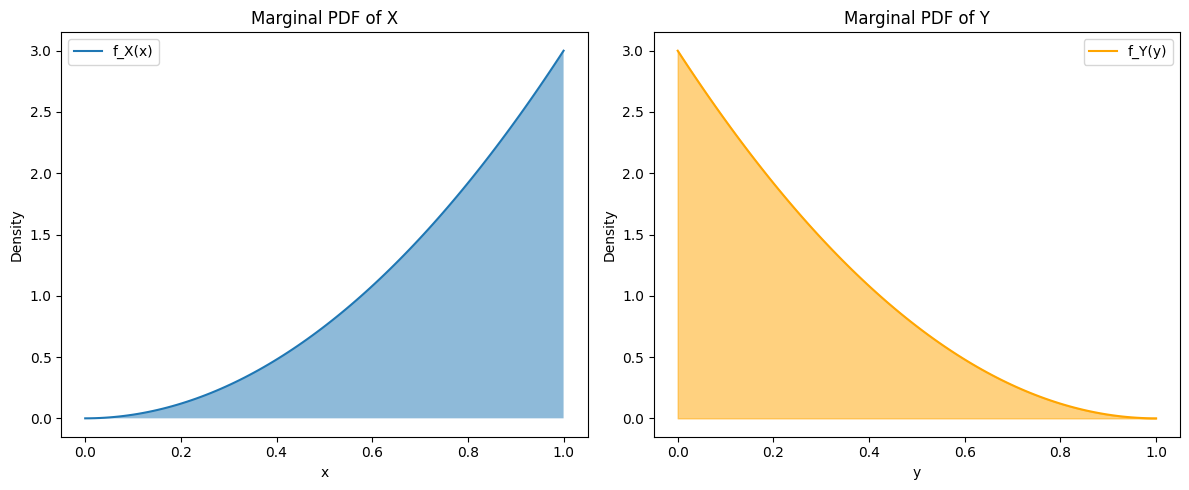
\includegraphics[width=0.8\textwidth]{img/XY.png}
  \caption{周辺確率密度関数}
  \label{fig:6_1}
\end{figure}
\( y \) については,\( 0 \leq y < x \) 以外で,被積分関数は 0 (\( x \) も同様) であることに注意して,
\begin{align*}
  g(x) & = \int_0^x 6(x - y)dy = 3x^2,      \\
  h(y) & = \int_y^1 6(x - y)dx = 3(1 - y)^2
\end{align*}
となる.
これらの密度関数は \( \frac{1}{2} \) について線対称である.

期待値は,
\begin{align*}
  E(X) & = \int_0^1 x \cdot g(x)dx = \int_0^1 x \cdot 3x^2 dx = \frac{3}{4},       \\
  E(Y) & = \int_0^1 y \cdot h(y)dy = \int_0^1 y \cdot 3(1 - y)^2 dy = \frac{1}{4}.
\end{align*}

\begin{align*}
  E(X^2) & = \int_0^1 x^2 \cdot 3x^2 dx = \frac{3}{5},        \\
  E(Y^2) & = \int_0^1 y^2 \cdot 3(1 - y)^2 dy = \frac{1}{10}.
\end{align*}

よって,分散は,
\begin{align*}
  V(X) & = \frac{3}{80}, \quad V(Y) = \frac{3}{80}.
\end{align*}

共分散は,
\begin{align*}
  \text{Cov}(X, Y) & = \frac{1}{5} - \frac{3}{4} \cdot \frac{1}{4} = \frac{1}{80}.
\end{align*}

相関係数は,
\begin{align*}
  \rho & = \frac{\frac{1}{80}}{\sqrt{\frac{3}{80}} \cdot \sqrt{\frac{3}{80}}} = \frac{1}{3}.
\end{align*}

\subsection{たたみこみの直接計算によって,上で挙げた分布の再生性を証明せよ.
  すなわち,$X, Y$ が独立で,\ref{6_2_1},\ref{6_2_2},\ref{6_2_3}を満たすことを証明せよ.}
\subsection*{ヒント:\ref{6_2_1}では式\eqref{6-2-1}に示すヴァンデルモンドのたたみこみ定理を用いると良い.
  また,\ref{6_2_3}では式\eqref{6-2-3}に示す指数部分が二次関数の一般形になる場合のガウス積分を用いると良い.}
\begin{align}
  \sum_{x=0}^{z} \binom{n}{x} \binom{m}{z-x}                     & = \binom{n+m}{z} \label{6-2-1}                                           \\
  \int_{-\infty}^{\infty} \exp\{-\left(ax^2 + bx + c\right)\} dx & = \exp\left(\frac{b^2}{4a} - c\right)\sqrt{\frac{\pi}{-a}} \label{6-2-3}
\end{align}
\subsubsection{$p$ が等しい二項分布に従うならば,$X + Y$ も二項分布に従う}\label{6_2_1}
\begin{align}
  Bi(n,p) * Bi(m,p) & = \sum_{x=0}^{z} \binom{n}{x} p^x q^{n-x} \cdot \binom{m}{z-x} p^{z-x} q^{m-(z-x)} \notag \\
                    & = \sum_{x=0}^{z} \binom{n}{x} \binom{m}{z-x} p^z q^{(n+m)-z} \notag                       \\
                    & = \binom{n+m}{z} p^z q^{(n+m)-z} \notag                                                   \\
                    & = Bi(n+m,p) \notag                                                                        \\
\end{align}
2行目から3行目への変換で,ヴァンデルモンドの畳み込み定理を用いた.
\subsubsection{ポアソン分布に従うならば,$X + Y$ もポアソン分布に従う}\label{6_2_2}
\begin{align}
  P_0(\lambda) * P_0(\mu) & = \sum_{x=0}^{z} \frac{e^{-\lambda} \lambda^x}{x!} \cdot \frac{e^{-\mu} \mu^{z-x}}{(z-x)!} \notag    \\
                          & = e^{-(\lambda+\mu)} \sum_{x=0}^{z} \frac{x!}{x! (z-x)!} \cdot \frac{\lambda^x \mu^{z-x}}{z!} \notag \\
                          & = e^{-(\lambda+\mu)} \cdot \frac{(\lambda + \mu)^z}{z!} \notag                                       \\
                          & = P_0(\lambda + \mu) \notag
\end{align}
\subsubsection{正規分布に従うならば,$X + Y$ も正規分布に従う}\label{6_2_3}
\begin{align}
  N(\mu_1, \sigma_1^2) + N(\mu_2, \sigma_2^2) & = \int_{-\infty}^{\infty} \frac{1}{\sqrt{2\pi\sigma_1^2}} e^{-\frac{(x-\mu_1)^2}{2\sigma_1^2}} \cdot \frac{1}{\sqrt{2\pi\sigma_2^2}} e^{-\frac{(z-x-\mu_2)^2}{2\sigma_2^2}} dx \notag \\
                                              & = \frac{1}{2\pi\sigma_1\sigma_2} \int_{-\infty}^{\infty} e^{-\left[ \frac{(x-\mu_1)^2}{2\sigma_1^2} + \frac{(z-x-\mu_2)^2}{2\sigma_2^2} \right]} dx \notag                            \\
\end{align}
ここで,指数部分について平方完成し,できた定数項を $z$ について平方完成すると,
\begin{align}
  \text{指数部分} & = \frac{\sigma_1^2 + \sigma_2^2}{2\sigma_1^2\sigma_2^2} \left[ x - \frac{\sigma_2^2\mu_1 + \sigma_1^2\mu_2}{\sigma_1^2+\sigma_2^2} \right]^2 - \frac{(z - (\mu_1+\mu_2))^2}{2(\sigma_1^2 + \sigma_2^2)} \notag \\
              & \text{よって、$N(\mu_1, \sigma_1^2) * N(\mu_2, \sigma_2^2)$ の式は、} \notag                                                                                                                                           \\
              & = \frac{1}{\sqrt{2\pi(\sigma_1^2 + \sigma_2^2)}} e^{-\frac{(z-(\mu_1+\mu_2))^2}{2(\sigma_1^2+\sigma_2^2)}} \notag                                                                                              \\
              & = N(\mu_1 + \mu_2, \sigma_1^2 + \sigma_2^2) \notag
\end{align}
\section{中心極限定理を証明せよ}%% 課題7
互いに独立な $n$ この確率変数 $X_1, X_2, \ldots, X_n$ が平均 $\mu$, 分散 $\sigma^2$ を持つ同一の確率分布に従うとする.
$n \to \infty$ のとき,
\[
  P \left( a \leq \frac{\overline{X} - \mu}{\sigma / \sqrt{n}} \leq b \right) \to \int_a^b \frac{1}{\sqrt{2\pi}} e^{-\frac{t^2}{2}} dt
  \quad \text{(ただし, } \overline{X} = \frac{1}{n}(X_1 + X_2 + \cdots + X_n) \text{)}
\]

左辺にある,$\overline{X}$ の標準化変数を変形すると,
\begin{align}
  \frac{X_1 + X_2 + \cdots + X_n - n\mu}{\sqrt{n} \sigma} = \frac{Y_1 + Y_2 + \cdots + Y_n}{\sqrt{n}}
\end{align}
の確率分布が,$n$ が大きいとき正規分布に近づくことを示せばよい.ここで,
\[
  Y_1 = \frac{X_1 - \mu}{\sigma}, \, Y_2 = \frac{X_2 - \mu}{\sigma}, \, \ldots, \, Y_n = \frac{X_n - \mu}{\sigma}
\]
は、それぞれ $X_1, X_2, \ldots, X_n$ の標準化変数であって,
\[
  E(Y_1) = E(Y_2) = \cdots = E(Y_n) = 0, \, V(Y_1) = V(Y_2) = \cdots = V(Y_n) = 1
\]
となっている.$X_1, X_2, \ldots, X_n$ の確率分布は全て同一であり,$Y_1, Y_2, \ldots, Y_n$ についてもそうであるから,その一つを $Y$ とおいてモーメント母関数を求める.1次のモーメント $\mu_1 = E(Y) = 0$, 2次のモーメント $\mu_2 = E(Y^2) = 1$ なので,
\[
  M_Y(t) = 1 + \frac{t^2}{2} + \cdots
\]

独立な確率変数の確率分布はモーメント母関数の積で求まるので,$Y_1 + Y_2 + \cdots + Y_n \equiv T$ モーメント母関数は,
\[
  M_n(t) = \left( M_Y(t) \right)^n = \left( 1 + \frac{t^2}{2} + \cdots \right)^n
\]

最後的に $\frac{Y_1 + Y_2 + \cdots + Y_n}{\sqrt{n}}$ のモーメント母関数は,$t = \frac{t}{\sqrt{n}}$ とおきかえて,
\[
  M_n \left( \frac{t}{\sqrt{n}} \right) = \left( M_Y \left( \frac{t}{\sqrt{n}} \right) \right)^n
  = \left( 1 + \frac{t^2}{2n} + \cdots \right)^n \to e^{\left( \frac{t^2}{2} \right)}
\]
$e^{\left( \frac{t^2}{2} \right)}$ は標準正規分布のモーメント母関数である.
\section{1袋50g入りの菓子製造工程において、製品10個を無作為に抽出し、重さを測定したところ、次のようになった。}%% 課題8
1 袋中の菓子の重さ(g):51.9, 49.5, 50.2, 50.3, 50.1, 52.1, 48.8, 48.5, 49.7, 49.6
\subsubsection{全製品の平均重量とその分散の不偏推定量を求めよ。}
平均重量は,
\begin{align}
  \overline{x} & = \frac{1}{10} \sum_i x_i = \frac{1}{10} \times 500.7 = 50.07
\end{align}
また,分散の不偏推定量は,
\begin{align}
  s^2 & = \frac{1}{10 - 1} \left( \sum (x_i^2) - n \overline{x}^2 \right) \\
      & = \frac{1}{10 - 1} \left( 25082.35 - 10 \times 50.07^2 \right)    \\
      & = 1.3668
\end{align}

\subsubsection{次ページ以降の数表を用いて、母平均$\mu$と母分散$\sigma^2$の 99$\%$信頼区間を求めよ。}
99\%信頼区間を求めるので,$\gamma = 0.99$ つまり,$\alpha = 1 - \gamma = 0.01$ である.母平均 $\mu$ について,
\[
  \overline{x} - t_{n-1}\left( \frac{\alpha}{2} \right) \sqrt{\frac{s^2}{n}}
  \leq \mu \leq
  \overline{x} + t_{n-1}\left( \frac{\alpha}{2} \right) \sqrt{\frac{s^2}{n}}
\]
を $t$ 分布の数表を用いて求めれば良い.

\[
  t_{n-1}\left( \frac{\alpha}{2} \right) = t_9(0.005) = 3.250
\]
\[
  t_{n-1}\left( \frac{\alpha}{2} \right) \sqrt{\frac{s^2}{n}}
  = 3.250 \times \sqrt{\frac{1.3668}{10}} = 1.2015
\]

従って,
\[
  \text{上側限界} = 50.07 + 1.2015 = 51.2715
\]
\[
  \text{下側限界} = 50.07 - 1.2015 = 48.8685
\]

以上より,母平均の99\%信頼区間は
\[
  48.87 < \mu < 51.27
\]

\subsection*{母分散について}
母分散 $\sigma^2$ について,
\[
  \frac{(n-1)s^2}{\chi^2_{n-1}\left( \frac{\alpha}{2} \right)}
  < \sigma^2 <
  \frac{(n-1)s^2}{\chi^2_{n-1}\left( 1 - \frac{\alpha}{2} \right)}
\]
を $\chi^2$ 分布の数表を用いて求めれば良い.

\[
  \chi^2_{n-1}\left( \frac{\alpha}{2} \right) = \chi^2_9(0.005) = 23.5894
\]
\[
  \chi^2_{n-1}\left( 1 - \frac{\alpha}{2} \right) = \chi^2_9(0.995) = 1.7349
\]

\[
  \frac{(n-1)s^2}{\chi^2_{n-1}\left( \frac{\alpha}{2} \right)}
  = \frac{9 \times 1.3668}{23.5894} = 0.5215
\]
\[
  \frac{(n-1)s^2}{\chi^2_{n-1}\left( 1 - \frac{\alpha}{2} \right)}
  = \frac{9 \times 1.3668}{1.7349} = 7.0904
\]

以上より母分散の99\%信頼区間は
\[
  0.52 < \sigma^2 < 7.09
\]
% 参考文献
% \begin{thebibliography}{99}
%   \bibitem{}
% \end{thebibliography}

\end{document}